\documentclass[11pt]{article}

\usepackage[a4paper,margin=2.5cm]{geometry}
\usepackage[T1]{fontenc}
\usepackage{lmodern}
\usepackage{microtype}
\usepackage{amsmath,amssymb,mathtools}
\usepackage{booktabs,tabularx,longtable,array}
\usepackage{graphicx}
\usepackage{tikz}
\usetikzlibrary{arrows.meta,positioning,fit,calc}
\usepackage[backend=biber,style=authoryear,natbib=true,maxcitenames=2,maxbibnames=20]{biblatex}
\addbibresource{references.bib}
\usepackage[hidelinks]{hyperref}
\usepackage[nameinlink,noabbrev]{cleveref}
\usepackage{enumitem}
\usepackage{xcolor}

\newcommand{\Jam}{\textsc{Jam}}
\newcommand{\Elves}{\textsc{Elves}}
\newcommand{\E}{\mathbb E}
\newcommand{\Prb}{\mathbb P}
\newcommand{\floor}[1]{\left\lfloor #1\right\rfloor}
\newcommand{\ceil}[1]{\left\lceil #1\right\rceil}

\title{\textbf{Correlated Honest Failure in JAM/ELVES}\\
\large Fault-Domain Concentration, Sampling Dilution, and Recurrent Corrective Capacity}
\author{Albert Jan van Hoek}
\date{Draft --- September 2026}

\begin{document}
\maketitle

\begin{abstract}
Execution-auditing protocols distinguish adversarial validators from honest validators, but implementation faults create a third class: validators that follow the protocol and nevertheless return the same wrong judgment on a particular crafted input. We extend the ELVES/JAM auditing model to this \emph{correlated honest failure} case and separate consequences that arise at different protocol layers and timescales.

First, the current JAM dispute rules imply an attribution boundary that does not depend on the ELVES adaptive-crash model. If a fraction \(\gamma\) of validators is adversarial and a fraction \(f\) of the otherwise-honest validators shares a fault that makes one invalid report appear valid, then the maximum wrong-positive share is \(p_x=\gamma+(1-\gamma)f\). A bad verdict---and therefore the Gray Paper's ordinary culprit/fault attribution path---remains available regardless of adversarial voting only while the independently correct share is at least the verdict quorum. Asymptotically this requires \(p_x<1/3\).

Second, under the ELVES pessimistic branching model, correlated honest failure changes the corrective reproduction mean from \(F(1-\gamma)\) to
\[
\lambda_x=F(1-\gamma)(1-f)=Fh_x,
\]
where \(h_x\) is the fraction of validators that are both non-adversarial and independently correct for fault \(x\). Supercritical correction requires \(\lambda_x>1\), giving \(f<1-1/[(1-\gamma)F]\). The tranche factor \(F\) therefore trades tolerance of fault-domain concentration against committee growth under no-shows.

Third, sampled correction breaks a monotonicity property that holds when every participant supplies an independent blocking route. Writing \(C_x\) for the number of independently correct validators in a population of size \(N\), \(\lambda_x=FC_x/N\). Adding honest validators outside \(C_x\) lowers \(\lambda_x\) even with no behavioral change. In an exact-count illustration based on \(N=1023\), \(205\) adversarial validators and \(164\) honest validators sharing one fault, adding 200 further honest validators with the same fault raises the pessimistic acceptance bound from \(4.5\times10^{-4}\) to \(0.13\) when the initial committee is held at 30; if JAM's 341 cores remain fixed so the initial sample grows with \(N\), the same bound still rises to \(0.087\).

Fourth, event-level corrective reproduction is not the same as reproduction of corrective capacity across audits. We introduce a minimal slow loop between independently corrective capacity, observability of genuine maintenance, and returned resources. For the canonical three-process cycle, Lean verifies the exact replacement boundary
\[
(1-r_C)(1-r_O)(1-r_R)\le k_{CO}k_{OR}k_{RC}.
\]
The fast condition \(\lambda_x>1\) and the strict slow-maintenance condition are logically independent; machine-checked witnesses inhabit all four fast/slow phase cells. Thus an audit can be supercritical today while the capacity required for future independent correction erodes, and a self-maintaining validator ecosystem can still be insufficiently independent for one fault.

These are model extensions, not claims about an observed JAM vulnerability. The attribution result follows from the current Gray Paper verdict rules; the branching, dilution, and slow-maintenance results inherit explicit modeling assumptions. The slow-loop coefficients are interface parameters for delegated staking, operator, client, and ecosystem functions, not measured JAM constants. The purpose is to make the additional assumptions required by correlated honest failure and recurrent corrective capacity explicit and reviewable by the ELVES and JAM authors.
\end{abstract}

\section{Introduction}

Efficient execution auditing relies on a deliberate asymmetry: only a small randomly selected subset of validators re-executes a report in the ordinary case, while additional validators are recruited if the first audit does not resolve cleanly. ELVES formalizes this architecture under Byzantine assumptions and adaptive crashes, and the JAM Gray Paper adopts an equivalent auditing-and-judging mechanism \citep{burdges2024,wood2026}.

The security argument therefore depends not only on the number of validators but on what fraction of the population can supply a correct independent judgment for the report being audited.

The usual honest/adversarial partition hides one important failure mode. A validator can be honest in the game-theoretic and protocol sense---it executes the assigned software, announces when selected, and publishes the result it obtains---yet still be wrong because several validators share the same implementation defect. This is a classical concern in multiversion software: independently developed implementations can exhibit coincident failures on the same inputs, and nominal redundancy does not by itself imply independent failure \citep{eckhardt1985,littlewood1989}.

JAM explicitly encourages implementation diversity, but the question studied here is narrower:

\begin{quote}
\textbf{What changes in the JAM/ELVES security bookkeeping when some otherwise-honest validators share a fault that makes one crafted invalid report appear valid?}
\end{quote}

We call this \emph{correlated honest failure}. The phrase is fault-specific. A validator class can be correct for almost all reports and correlated only on one input family. Consequently the relevant quantity is not the number of clients but the size of a \emph{fault domain}: the set of validators that would produce the same erroneous judgment for the same fault.

This paper separates three layers that should not be conflated.

\begin{enumerate}[label=\textbf{R\arabic*.},leftmargin=*]
\item \textbf{Verdict attribution.} Given the current Gray Paper dispute rules, how large can the combined adversarial-plus-buggy-positive bloc become before a bad verdict, and therefore ordinary offender attribution, can no longer be guaranteed?
\item \textbf{Audit escalation.} Under ELVES's pessimistic adaptive-crash branching model, how does a shared fault change the reproduction number of independent correction?
\item \textbf{Sampling dilution.} When only a sample audits, can adding honest-but-correlated validators reduce structural safety even before incentives or behavior change?
\end{enumerate}

The first result is the strongest because it depends only on the current JAM verdict rules plus the correlated-fault thought experiment. The second and third results are extensions of ELVES and inherit its modeling assumptions.

\subsection{Main results}

Let \(N\) be the verdict validator-set size. Let \(A\) validators be adversarial, \(B_x\) otherwise-honest validators share fault \(x\) and judge one invalid report as valid, and \(C_x=N-A-B_x\) independently judge it as invalid. Define
\[
\gamma=\frac{A}{N},
\qquad
f_x=\frac{B_x}{N-A},
\qquad
p_x=\frac{A+B_x}{N}=\gamma+(1-\gamma)f_x.
\]

The Gray Paper requires each verdict to contain
\[
K=\floor{\frac{2N}{3}}+1
\]
judgments. A bad verdict contains zero positive judgments. It can therefore be formed despite the adversary voting positive if and only if
\[
\boxed{C_x\ge K.}
\]
For large \(N\), this is
\[
\boxed{p_x<\frac13.}
\]
At the other end, a good verdict becomes constructible if \(A+B_x\ge K\), asymptotically \(p_x>2/3\).

In the ELVES branching extension, only \(C_x/N\) supplies independent honest correction, so
\[
\boxed{\lambda_x=F\frac{C_x}{N}=F(1-\gamma)(1-f_x).}
\]
Supercritical correction requires \(\lambda_x>1\). Thus the fault-domain criticality boundary is
\[
\boxed{
 f_{\rm crit}=1-\frac{1}{(1-\gamma)F}.
}
\]
For JAM's current \(F=2\), the asymptotic boundaries are particularly transparent in terms of \(p_x\):
\[
\boxed{
\underbrace{\frac13}_{\text{bad-verdict attribution}}
<
\underbrace{\frac12}_{\text{audit escalation}}
<
\underbrace{\frac23}_{\text{false-good eligibility}}.
}
\]
The ordering is illustrated in \Cref{fig:thresholds}.

Finally, with \(C_x\) fixed,
\[
\lambda_x(N)=F\frac{C_x}{N}
\]
is strictly decreasing in \(N\). Hence adding honest validators that belong to the same fault domain can reduce the corrective reproduction number without any behavioral response. The effect remains in a JAM-specific fixed-core variant in which the expected initial sample grows with validator count, although the larger sample partly offsets the dilution.

\subsection{Scope}

Nothing in this paper establishes that JAM currently violates a security requirement or that a particular correlated client bug exists. The model deliberately asks what follows \emph{if} a crafted report lies inside a shared fault domain. The results are therefore best read as assumption audits and design margins.

The paper also distinguishes accidental failure from strategic exploitation. For an accidental bug, assignment probabilities determine how often a bad report is produced and how often independently correct auditors see it. For a strategic attacker who knows the bug, opportunity can be concentrated on favorable assignments. We quantify the frequency of such assignments but do not assume the attacker can route arbitrary work to a chosen core unless that ability is established separately.

\section{Protocol elements and model}
\label{sec:model}

\subsection{JAM auditing and disputes}

The current Gray Paper states that JAM's auditing and judging system is theoretically equivalent to ELVES \citep{wood2026,burdges2024}. Each validator initially audits a random deterministic selection of up to ten active cores. If an announced auditor fails to produce a positive judgment, later tranches recruit additional auditors. The Gray Paper sets the audit bias factor to
\[
F=2,
\]
meaning that one unmatched announcement induces an expected two additional auditors in the next tranche. A negative judgment instead causes broad re-auditing and opens the dispute path.

The dispute rules are central to our first result. Let
\[
K=\floor{\frac{2N}{3}}+1
\]
be the number of judgments carried by a verdict and
\[
W=\floor{\frac{N}{3}}
\]
the number of positive judgments required for a wonky verdict. Under the current Gray Paper rule, a verdict is:
\begin{itemize}
\item \textbf{good} if all \(K\) included judgments are positive;
\item \textbf{bad} if all \(K\) included judgments are negative;
\item \textbf{wonky} if exactly \(W\) of the \(K\) judgments are positive.
\end{itemize}

Bad and wonky verdicts remove the availability assignment. The Gray Paper's ordinary offense paths are tied to good or bad reports: guarantors of a bad report can be included as culprits, and judges contradicting an established good/bad verdict can be included as faults. A wonky report is recorded in the wonky set, but the current specification does not place its guarantors or judges in the punish set through those culprit/fault rules \citep{wood2026}.

This paper therefore uses the precise phrase \emph{protocol-defined offender attribution path} rather than equating a wonky verdict with zero economic consequences. A staking subsystem could in principle react to the wonky record; the Gray Paper leaves validator rewards and much of the higher-level economics outside the JAM chain itself.

\subsection{ELVES branching quantities}

ELVES models the audit-tranche process with a pessimistic adaptive-crash adversary. Let \(s_0\) be the expected initial audit committee and let \(F\) be the expected number of auditors recruited per unmatched prior auditor. If a fraction \(\gamma\) of the validator population is adversarial, the mean number of useful honest offspring in the branching approximation is
\[
\lambda=(1-\gamma)F.
\]
If \(q\) is the extinction probability of the corresponding Poisson Galton--Watson process, then
\[
q=\exp[-\lambda(1-q)],
\]
and the ELVES soundness analysis yields the pessimistic acceptance bound
\[
\boxed{
P_{\rm accept}\le q^{s_0/F}.
}
\]
Useful escalation requires \(\lambda>1\).

The same architecture has a no-show/scalability side. If \(u\) is the fraction represented in the no-show/fault-amplification term, the reproduction number is \(uF\), so the static expected-final-committee bound has the form
\[
\boxed{
 s_f\le\frac{s_0}{1-uF},
 \qquad uF<1.
}
\]
ELVES reports a continuous-model optimum near \(F=2.0794\) under its stated assumptions; the Gray Paper uses \(F=2\).

\subsection{Correlated honest fault domain}

For one crafted invalid report and one fault class \(x\), partition the verdict population into:
\begin{align*}
A &: \text{adversarial validators},\\
B_x &: \text{otherwise-honest validators that judge the invalid report as valid},\\
C_x &: \text{otherwise-honest validators that independently judge it as invalid}.
\end{align*}
Thus
\[
N=A+B_x+C_x.
\]

The central distinction is:
\[
\boxed{
\text{honest validator count}
\neq
\text{fault-specific independently corrective validator count}.
}
\]

When convenient we write
\[
\gamma=\frac{A}{N},
\qquad
f_x=\frac{B_x}{N-A},
\]
so
\[
\frac{C_x}{N}=(1-\gamma)(1-f_x).
\]
The parameter \(f_x\) should not be interpreted as a universal client market share. It is the exposure of honest validators to fault \(x\). A client implementation is one possible fault domain, but shared libraries, compilers, virtual machines, cryptographic code, erasure-coding implementations, or copied specification logic can couple nominally distinct clients.

\subsection{Claim-status map}

\begin{table}[htbp]
\centering
\small
\caption{Status of the main claims. Extension means derived after changing an ELVES/JAM assumption; it is not attributed to the original authors.}
\label{tab:claims}
\begin{tabularx}{\textwidth}{@{}p{0.05\textwidth}X p{0.23\textwidth}@{}}
\toprule
ID & Claim & Status \\
\midrule
A1 & A bad verdict remains constructible against adversarial positive voting iff \(C_x\ge K\). & Exact consequence of Gray Paper verdict rule + declared fault model \\
A2 & A good verdict becomes constructible if \(A+B_x\ge K\). & Exact consequence of Gray Paper verdict rule + declared fault model \\
A3 & For large \(N\), robust bad-verdict attribution requires \(\gamma+(1-\gamma)f_x<1/3\). & Asymptotic form of A1 \\
B1 & Correlated honest failure changes the ELVES corrective mean to \(\lambda_x=F C_x/N\). & ELVES extension \\
B2 & Supercritical correction requires \(f_x<1-1/[(1-\gamma)F]\). & Exact consequence of B1 \\
B3 & Increasing \(F\) raises fault-domain tolerance while worsening the static no-show committee bound. & ELVES extension / comparative result \\
C1 & Holding \(C_x\) fixed, adding validators outside the independently correct set strictly lowers \(\lambda_x=FC_x/N\). & Exact sampling identity \\
C2 & In the declared baseline, the pessimistic acceptance bound worsens under such additions both for fixed \(s_0=30\) and fixed 341 cores. & Computational specialization \\
D1 & Slashable collateral need not be attacker-attributable collateral under an honest shared bug. & Economic mapping observation; not a theorem of JAM \\
D2 & Guarantor diversity, effort proofs, announcement monitoring and load feedback are design questions, not established fixes. & Hypotheses / future work \\
\bottomrule
\end{tabularx}
\end{table}

\section{Result 1: fault-domain concentration creates an attribution boundary}
\label{sec:attribution}

This result uses only the Gray Paper verdict composition rules plus the fault-domain model in \Cref{sec:model}. It does not use the ELVES adaptive-crash branching approximation.

\subsection{Exact finite-population verdict conditions}

Suppose enough judgments eventually exist to construct a verdict. Let \(P\) be the number of validators that would issue a positive judgment for the invalid report and \(N-P\) the number issuing a negative judgment.

A bad verdict can be constructed if and only if at least \(K\) negative judgments are available:
\[
\boxed{
N-P\ge K.
}
\]
A good verdict can be constructed if and only if
\[
\boxed{
P\ge K.
}
\]
A wonky verdict can be constructed if and only if at least \(W\) positive and \(K-W\) negative judgments are available:
\[
\boxed{
P\ge W
\quad\text{and}\quad
N-P\ge K-W.
}
\]
These are selection conditions: a block author can choose the required \(K\) signed judgments from the available pool.

For JAM's current \(N=1023\),
\[
K=683,
\qquad
W=341,
\qquad
K-W=342.
\]
Therefore:
\begin{itemize}
\item a bad verdict is possible for \(P\le340\);
\item a wonky verdict is possible for \(341\le P\le681\);
\item a good verdict is possible for \(P\ge683\).
\end{itemize}

Under the literal current rule, \(P=682\) is a one-vote edge case in which none of the three allowed positive counts can be selected from a 683-judgment verdict: there are only 341 negatives, too few for the wonky composition, but only 682 positives, too few for a good verdict. We treat this as a specification question for the JAM authors rather than silently smoothing it away.

\subsection{Robust bad-verdict attribution}

Under correlated honest failure, honest buggy validators contribute positive judgments, honest independent validators contribute negative judgments, and adversarial validators may choose either sign.

To prevent a bad verdict, the adversary's best choice is to vote positive. The maximum positive population is then
\[
P_{\max}=A+B_x,
\]
and the remaining negative population is \(C_x\).

Hence a bad verdict remains available regardless of adversarial voting if and only if
\[
\boxed{
C_x\ge K.
}
\]
Equivalently,
\[
A+B_x\le N-K.
\]

Writing
\[
p_x=\frac{A+B_x}{N}=\gamma+(1-\gamma)f_x,
\]
the large-\(N\) form is
\[
\boxed{p_x<\frac13.}
\]
Solving for \(f_x\) gives
\[
\boxed{
 f_x<\frac{1/3-\gamma}{1-\gamma},
}
\]
when \(\gamma<1/3\).

At \(\gamma=0.2\), the asymptotic limit is
\[
f_x<\frac{1/3-0.2}{0.8}=\frac16\approx0.167.
\]
Thus a shared fault affecting roughly one-sixth of the honest population can consume the entire remaining one-third attribution budget when the adversarial share is 20\%.

The interpretation is narrow but important. Below this boundary, independently correct honest validators alone supply enough negative judgments for a bad verdict. Above it, the adversary can prevent a bad verdict simply by joining the buggy positive bloc.

\subsection{The wonky region}

Suppose
\[
A+B_x\ge W
\]
but independently correct negative validators are still numerous enough for the wonky composition:
\[
C_x\ge K-W.
\]
Then an adversary voting positive can make a wonky verdict constructible while preventing a bad verdict.

Under the current Gray Paper, a wonky verdict is non-positive and therefore stops the report from proceeding, but the culprit/fault rules do not create ordinary offender records for wonky reports. Thus the system can remain \emph{safety preserving at the report level} while losing the ordinary attribution path.

This is the first important separation:
\[
\boxed{
\text{report rejection}
\neq
\text{offender attribution}.
}
\]

It is deliberately not stated as “the attacker pays nothing.” The staking layer may define additional consequences for wonky records. The Gray Paper does not specify such a rule, so whether wonky is economically cost-free is an explicit question for the JAM/Polkadot staking design.

\subsection{Strategic choice inside the intermediate region}

There is a second asymmetry. If the honest buggy population by itself is still small enough that
\[
B_x\le N-K,
\]
the adversary can instead vote negative. Then at least \(K\) negative judgments may be available, making a bad verdict constructible. In that branch the honest buggy validators' positive judgments contradict the bad verdict and their guarantor/judgment signatures may become offender evidence, whereas adversarial validators that voted negative do not contradict it.

Thus in part of the intermediate region the adversary can choose between two qualitatively different protocol outcomes:
\begin{enumerate}[label=(\alph*)]
\item vote positive, preventing a bad verdict and steering toward wonky; or
\item vote negative, permitting a bad verdict whose fault attribution can fall on honest buggy validators.
\end{enumerate}

This does not prove an attacker can always avoid all economic loss, because entering the pipeline may itself require attacker-controlled signatures or other costs. It shows that the verdict layer does not by itself force the collateral cost to fall on the party exploiting the shared fault.

\subsection{False-good eligibility}

If
\[
A+B_x\ge K,
\]
then a good verdict becomes constructible when the adversarial and buggy-positive blocs align. Asymptotically,
\[
\boxed{p_x>\frac23.}
\]
For \(\gamma=0.2\), this occurs at approximately
\[
f_x>\frac{2/3-0.2}{0.8}\approx0.583.
\]
At that point the dispute layer itself can accept the invalid report as good under the fault model, and correct negative judges fall on the dissenting side of the protocol verdict.

\subsection{Threshold ordering}

For JAM's \(F=2\), \Cref{sec:escalation} will show that the ELVES corrective branching process loses supercriticality at
\[
p_x=1-\frac1F=\frac12.
\]
The three large-population boundaries are therefore ordered as
\[
\boxed{
\frac13
<
\frac12
<
\frac23.
}
\]

\begin{figure}[htbp]
\centering
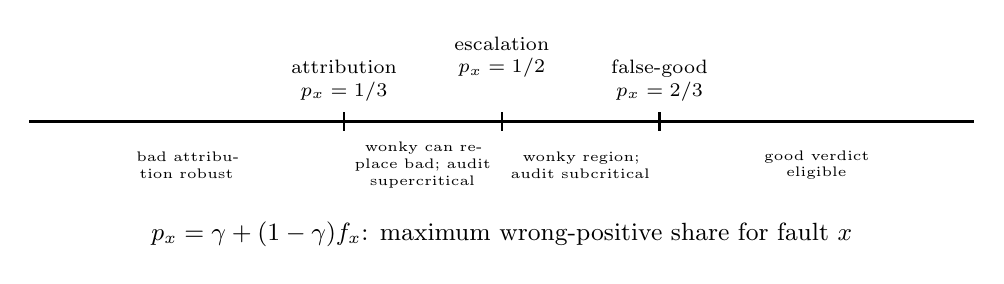
\begin{tikzpicture}[x=12cm,y=1cm,>=Latex,font=\small]
\draw[very thick] (0,0) -- (1,0);
\foreach \x in {0.333,0.5,0.667} {\draw[thick] (\x,0.12) -- (\x,-0.12);}
\node[align=center,font=\scriptsize] at (0.333,0.52) {attribution\\$p_x=1/3$};
\node[align=center,font=\scriptsize] at (0.5,0.82) {escalation\\$p_x=1/2$};
\node[align=center,font=\scriptsize] at (0.667,0.52) {false-good\\$p_x=2/3$};

\node[align=center,text width=1.7cm,font=\tiny] at (0.166,-0.55)
  {bad attribution robust};
\node[align=center,text width=1.8cm,font=\tiny] at (0.416,-0.55)
  {wonky can replace bad; audit supercritical};
\node[align=center,text width=1.8cm,font=\tiny] at (0.583,-0.55)
  {wonky region; audit subcritical};
\node[align=center,text width=1.7cm,font=\tiny] at (0.833,-0.55)
  {good verdict eligible};
\node[below=1.15cm] at (0.5,0)
  {$p_x=\gamma+(1-\gamma)f_x$: maximum wrong-positive share for fault $x$};
\end{tikzpicture}

\caption{Large-population fault-domain regimes for JAM's current \(F=2\). The first boundary concerns robust availability of a bad verdict and the ordinary offender-attribution path. The second is the ELVES-extension branching threshold. The third is eligibility for a good verdict under aligned adversarial and buggy-positive judgments. Exact finite-\(N\) rules use \(K=\floor{2N/3}+1\) and \(W=\floor{N/3}\).}
\label{fig:thresholds}
\end{figure}

At \(\gamma=0.2\), expressed as buggy share among otherwise-honest validators, these correspond approximately to 16.7\%, 37.5\%, and 58.3\% respectively.

\subsection{Offline validators tighten the attribution condition}

The verdict rule depends on available signed judgments, not only nominal validator identities. Let \(O\) validators be offline and unable to judge, disjoint from the adversarial and correlated-fault classes for this extension. Let \(f_x\) now denote the buggy share among the remaining non-adversarial online validators. The independently correct online share is
\[
\frac{C_x}{N}=(1-\gamma-o)(1-f_x),
\qquad o=\frac{O}{N}.
\]
A bad verdict robust to adversarial positive voting requires
\[
\boxed{
(1-\gamma-o)(1-f_x)\ge\frac{K}{N},
}
\]
which approaches
\[
(1-\gamma-o)(1-f_x)>\frac23.
\]
Offline capacity therefore consumes the same finite pool of negative judgments needed for attribution. This extension should not be conflated with ELVES no-shows: a validator that never announces an audit is not the same event as an announced auditor failing to return a judgment.

\section{Result 2: fault-specific corrective escalation}
\label{sec:escalation}

The attribution result above is a JAM verdict-layer statement. We now extend the ELVES branching model itself.

\subsection{Effective honest correction}

ELVES's honest offspring mean is
\[
\lambda=(1-\gamma)F.
\]
That expression treats every non-adversarial auditor as capable of identifying the invalid report. Under fault \(x\), only the independently correct class \(C_x\) supplies useful corrective offspring. We therefore replace the honest share by
\[
h_x=\frac{C_x}{N}=(1-\gamma)(1-f_x).
\]
The fault-specific reproduction mean is
\[
\boxed{
\lambda_x=Fh_x=F(1-\gamma)(1-f_x).
}
\]
This is an extension of ELVES, not a result stated in \citet{burdges2024}.

The branching process remains supercritical only if
\[
\lambda_x>1,
\]
so
\[
\boxed{
 f_x< f_{\rm crit}
 =1-\frac{1}{(1-\gamma)F}.
}
\]

For \(F=2\):
\begin{center}
\begin{tabular}{ccc}
\toprule
Adversarial share \(\gamma\) & \(f_{\rm crit}\) & Interpretation \\
\midrule
\(1/3\) & 0.250 & 25\% of honest validators \\
0.20 & 0.375 & 37.5\% of honest validators \\
0.05 & 0.474 & 47.4\% of honest validators \\
\bottomrule
\end{tabular}
\end{center}

The concentration boundary should be interpreted as a \emph{fault-domain} limit, not a client-count rule. Client deployment share is an observable proxy only when the client is the relevant common failure domain.

\subsection{Target-specific margin}

Structural supercriticality is weaker than satisfying a quantitative soundness target. Let \(q_x\) solve
\[
q_x=\exp[-\lambda_x(1-q_x)]
\]
for \(\lambda_x>1\). Then the extended pessimistic bound is
\[
P_x\le q_x^{s_0/F}.
\]

ELVES Corollary 1 provides an economically derived target of the form
\[
\varepsilon_* = \frac{\nu}{N+\nu},
\]
when collateral is parameterized by \(\nu\) in the stated expected-profit argument. Inverting the branching bound for target \(\varepsilon\) gives
\[
q_* = \varepsilon^{F/s_0},
\qquad
\lambda_*=-\frac{\ln q_*}{1-q_*},
\]
and therefore
\[
\boxed{
 f_{\max}
 =1-\frac{\lambda_*}{(1-\gamma)F},
}
\]
provided the baseline \(f_x=0\) already meets the target.

For \(N=1023\), \(s_0=30\), \(F=2\), and illustrative \(\nu=0.05\), the target is not certified at the \(\gamma\to1/3\) boundary even at \(f_x=0\). At \(\gamma=0.20\), the bound certifies only about \(f_x\le0.146\); at \(\gamma=0.05\), about \(f_x\le0.280\). These numbers are certificate margins of the extended pessimistic model, not exact protocol frontiers.

\subsection{The tranche factor trades concentration tolerance against escalation load}

Increasing \(F\) raises \(\lambda_x\) and therefore tolerates a larger correlated-fault domain. But the ELVES static committee-size bound under a no-show/fault share \(u\) is
\[
 s_f\le\frac{s_0}{1-uF}.
\]
Thus the same parameter reduces distance to no-show explosion.

For \(s_0=30\) and \(u=0.30\):

\begin{table}[htbp]
\centering
\caption{Illustrative two-sided effect of the tranche factor. The client/fault thresholds are from the correlated-honest extension; the committee bound is the ELVES static form evaluated at \(u=0.30\).}
\label{tab:Ftradeoff}
\begin{tabular}{rrrr}
\toprule
\(F\) & \(f_{\rm crit}\), \(\gamma=1/3\) & \(f_{\rm crit}\), \(\gamma=0.20\) & \(s_f\) bound \\
\midrule
2.00 & 25.0\% & 37.5\% & 75 \\
2.0794 & 27.9\% & 39.9\% & 79.7 \\
2.50 & 40.0\% & 50.0\% & 120 \\
2.90 & 48.3\% & 56.9\% & 230.8 \\
\bottomrule
\end{tabular}
\end{table}

With \(s_0=30\) and \(\gamma=1/3\), the pessimistic acceptance bound is approximately \(1.13\times10^{-4}\) at \(F=2\) and \(4.54\times10^{-5}\) at ELVES's reported continuous optimum \(F\approx2.0794\), a ratio of about 2.49. This is a comparison of one modeled bound, not a statement that JAM is “2.5 times less secure.”

The design implication is simply that \(F\) sits between two margins:
\[
\boxed{
\text{corrective reproduction}
\quad\text{and}\quad
\text{failure/no-show reproduction}.
}
\]
If correlated honest failure is admitted to the threat model, the objective used to select \(F\) changes.

\section{Result 3: sampled correction breaks structural monotonicity}
\label{sec:sampling}

The preceding result can be written without separating adversarial and buggy shares:
\[
\boxed{
\lambda_x=F\frac{C_x}{N},
}
\]
where \(C_x\) is the number of validators that independently judge fault \(x\) correctly.

This form exposes a structural effect of sampling.

\subsection{Dilution theorem}

Hold \(F>0\) and \(C_x>0\) fixed. Add \(m>0\) validators that do not increase the independently correct set for fault \(x\). The new population is \(N'=N+m\) and
\[
\lambda_x' = F\frac{C_x}{N+m}.
\]
Then
\[
\boxed{
\lambda_x'<\lambda_x.
}
\]
No behavioral response is involved. Every added validator can be honest in the ordinary sense; the effect arises because committee membership is sampled from a larger population while the number of useful correctors for this fault does not increase.

This corrects the scope of a monotonicity result that holds in an all-participant coverage model. If every participant adds a blocking route, adding participants cannot reduce structural coverage. In sampled correction, an entrant can instead dilute the probability that a scarce corrective type enters the committee.

\subsection{Exact-count illustration}

To avoid ambiguity from rounded shares, take the baseline
\[
N_0=1023,
\qquad
A=205,
\qquad
B_x=164,
\qquad
C_x=654.
\]
Thus the baseline adversarial fraction is \(205/1023\approx0.2004\), while \(164/818\approx0.2005\) of the otherwise-honest validators belong to the fault domain.

Now add \(m\) honest validators that share the same fault, holding \(A\) and \(C_x\) fixed. This deliberately makes the adversarial fraction \emph{fall} as the population grows. Nevertheless \(C_x/N\) declines.

We evaluate two population-update variants.

\paragraph{Variant 1: fixed initial sample.}
Hold \(s_0=30\), \(F=2\). This isolates pure dilution.

\paragraph{Variant 2: fixed 341 JAM cores.}
The Gray Paper sets \(341\) cores as a separate constant and each validator initially samples ten active cores. Once all 341 cores are active, the expected initial auditors per report scale approximately as
\[
 s_0(N)=\frac{10N}{341}.
\]
This growing initial sample partly compensates dilution.

\begin{table}[htbp]
\centering
\small
\caption{Pessimistic ELVES-extension bound under fault-domain dilution. Added validators are honest but belong to the same fault domain. \(A=205\) and \(C_x=654\) remain fixed.}
\label{tab:dilution}
\begin{tabular}{rrrrr}
\toprule
Added buggy honest & \(N\) & \(\lambda_x\) & fixed \(s_0=30\) & fixed 341 cores \\
\midrule
0   & 1023 & 1.279 & \(4.52\times10^{-4}\) & \(4.52\times10^{-4}\) \\
100 & 1123 & 1.165 & \(9.12\times10^{-3}\) & \(5.76\times10^{-3}\) \\
200 & 1223 & 1.070 & 0.130 & 0.0874 \\
400 & 1423 & 0.919 & 1 & 1 \\
\bottomrule
\end{tabular}
\end{table}

The larger sample in the fixed-core case helps, but it does not eliminate the effect in this slice. At \(m=400\), \(\lambda_x<1\), so the pessimistic branching process is subcritical regardless of the larger initial sample.

This example should not be read as a forecast for validator-set growth. It is a structural counterexample to the proposition that adding honest validators necessarily improves sampled correction.

\subsection{Validator growth depends on how cores scale}

A related but distinct question is how the initial sample required by the ELVES economic target changes with \(N\). With \(F\), \(\gamma\), and collateral parameter \(\nu\) fixed, the target
\[
\varepsilon_* = \frac{\nu}{N+\nu}
\]
tightens roughly as \(1/N\). Because the branching bound is exponential in \(s_0\), the required initial sample grows only logarithmically in \(N\).

For \(F=2\), \(\gamma=1/3\), and \(\nu=0.05\), the required \(s_0\) is approximately:
\begin{center}
\begin{tabular}{rrrr}
\toprule
\(N\) & required \(s_0\) & if cores scale as \(N/3\) & if cores stay at 341 \\
\midrule
1023 & 32.8 & 30 & 30.0 \\
3000 & 36.3 & 30 & 88.0 \\
6000 & 38.6 & 30 & 176.0 \\
\bottomrule
\end{tabular}
\end{center}

Therefore the earlier shorthand “JAM fixes the sample at 30” is only true under a design in which core count continues to scale approximately as \(N/3\). Under the current Gray Paper's fixed 341-core constant, the expected sample per report instead grows linearly with validator count and rapidly exceeds this logarithmic requirement. The scaling concern is conditional on how a future system grows cores relative to validators.

\section{Corollaries and design questions}
\label{sec:implications}

The three main results are analytical. The following items are consequences or engineering questions, not recommendations established by the model.

\subsection{Slashable collateral is not necessarily attacker-attributable collateral}

ELVES's rational-adversary argument makes invalid acceptance prohibitively expensive by charging collateral to the attack path \citep{burdges2024}. In a conventional attack, the parties signing or backing an invalid result can be economically aligned with the attacker.

A shared implementation bug changes that mapping. If otherwise-honest guarantors compute the same wrong result and sign it, a later bad verdict can place \emph{their} signatures in the culprit path. The protocol may destroy collateral, yet the actor that selected the crafted input may not bear that loss.

The distinction is:
\[
\boxed{
\text{slashable collateral}
\neq
\text{attacker-attributable collateral}.
}
\]

This does not prove that exploiting the bug is cost-free. It means that the specific expected-profit argument needs an additional mapping from protocol offender to economic beneficiary when honest common-mode faults are admitted.

The wonky region strengthens the issue: the current Gray Paper does not create ordinary culprit/fault offender records for wonky reports. Whether the staking layer imposes a cost on a wonky report is therefore a first-order question for the protocol authors.

\subsection{Guarantor diversity as a design hypothesis}

Every active core has three assigned guarantors and a guarantee carries two or three credentials. If a single fault domain occupies population share \(r\), the probability that at least two of three randomly assigned guarantors belong to that domain is
\[
\Prb(\ge2)=3r^2(1-r)+r^3.
\]
At \(r=0.2\), this is \(0.104\). Across 341 cores, the expectation is approximately 35.5 core assignments per rotation with at least two guarantors from that domain.

This number does \emph{not} establish that an attacker can route a crafted package to one of those cores. It quantifies the frequency of favorable assignments if exploitation opportunities can be targeted or waited for.

One possible mitigation is to require the credential set for a guarantee to span declared implementation/fault-domain classes. This could prevent a single honest client bug from supplying both signatures. But the idea has unresolved issues:
\begin{itemize}
\item implementation identity may be self-declared and therefore gameable;
\item nominally distinct clients can share deeper components;
\item diversity constraints may reduce liveness when one implementation class is unavailable;
\item an adversarial validator can lie about identity, although doing so may force its own signature onto the report.
\end{itemize}
Hence guarantor diversity is a hypothesis to analyse, not a proposed protocol change in this paper.

\subsection{Fault-domain exposure metrics}

The quantity that matters for an unknown future bug cannot be measured directly: by definition we do not know which validators will be wrong on an input not yet discovered.

What can be measured is \emph{exposure} to shared components. Examples include validator share by:
\begin{itemize}
\item client implementation;
\item execution VM;
\item compiler/toolchain;
\item cryptographic or erasure-coding library;
\item major shared dependencies;
\item copied or common code paths.
\end{itemize}

These are upper bounds or proxies for possible fault-domain concentration, not measurements of \(f_x\) for an unknown bug. A useful operational question is therefore whether the largest identifiable shared-component exposure leaves adequate margin below the attribution and escalation boundaries.

\subsection{Announcement shortfall as an early-warning statistic}

JAM's later tranches respond to unmatched announcements. A validator that is offline before announcing is different: it simply reduces the number of initial auditors that appear.

Aggregate announcement counts per report can therefore serve as a statistical early-warning signal for loss of available corrective capacity. The expected count is known from validator count and active-core configuration. A sustained shortfall can indicate that the online population is smaller than the nominal population.

This is not a deterministic fault detector. Audit assignment is random, observations are local before information propagates, and the current formal validator-statistics tuple does not directly expose a finalized audit-count metric. The proposal is simply to monitor the discrepancy between expected and observed audit participation.

\subsection{Rubber-stamping remains an open interface}

The Gray Paper notes that auditing activity is difficult to track directly and delegates validator rewards to a staking subsystem; peer voting on impressions of validator effort is described as the available oracle mechanism \citep{wood2026}.

That leaves a classic verifier's-dilemma-style question \citep{luu2015}: how strongly does the reward signal discriminate actual re-execution from a validator that produces the expected positive judgment without paying the full computation cost?

The present paper does not claim that rubber-stamping is selected in JAM. The reward function and effort-observability mechanism are not sufficiently specified to close that game numerically. Candidate approaches such as verifiable execution artifacts, occasional test reports, or other proof-of-effort mechanisms should therefore be evaluated only after the actual staking design is specified.

\subsection{Load-dependent no-shows are a separate future model}

ELVES treats the no-show/fault share used in its committee-size analysis as exogenous. In a real implementation, no-show probability could rise with audit load. If
\[
u=u(L),
\]
and load \(L\) grows with the final committee size, then
\[
 s_f\approx\frac{s_0}{1-Fu(s_f)}
\]
becomes a feedback equation. This could amplify load under stress, but no claim of a JAM overload transition is made without empirical measurements of \(u(L)\). A testnet stress experiment measuring deadline misses against concurrent audit load would be the appropriate next step.

\section{Limitations and questions for the ELVES/JAM authors}
\label{sec:limitations}

The purpose of this paper is to expose assumptions, not to claim a complete security analysis. Several issues require author or implementation review.

\subsection{Correlated honest failure is outside the ELVES proof model}

The branching extension assumes that a buggy honest auditor behaves like an auditor that cannot produce a useful negative judgment for fault \(x\). This is a natural substitution in the reproduction mean, but it is not proved by ELVES. The exact coupling to adaptive crashes, tranche timing, and the paper's stronger committee-size concentration bounds should be checked by the ELVES authors.

\subsection{The verdict analysis assumes enough judgments become available}

The finite-population verdict conditions in \Cref{sec:attribution} concern which signed judgment compositions can be assembled. If too many validators are offline, a verdict may fail to reach \(K\) total judgments at all. That is a distinct liveness failure.

\subsection{What does the staking layer do with wonky?}

This is the highest-priority clarification.

The Gray Paper records wonky reports in a dedicated set and removes non-positive reports from the availability path. Its ordinary culprit/fault rules refer to good or bad reports, and its punish set is populated by those offense extrinsics. However, the chain's validator rewards and higher-level economic policy are delegated.

Therefore the paper's narrow claim is:
\begin{quote}
A wonky verdict does not create the ordinary Gray-Paper culprit/fault offender record.
\end{quote}
It does \emph{not} follow that a production staking system must impose zero cost. If the staking layer explicitly penalizes guarantors or judges associated with wonky, the economic attribution gap narrows.

\subsection{The one-vote finite-population gap}

At \(N=1023\), a global composition of 682 positive and 341 negative judgments does not appear to contain a valid 683-judgment subset with any of the three permitted positive counts \(683\), \(341\), or \(0\). This may be resolved elsewhere in the intended protocol semantics, or it may be an unreachable/irrelevant edge case under assumptions not represented in our abstraction. It should be confirmed rather than silently approximated by the continuous \(2/3\) boundary.

\subsection{Strategic entry is not established}

The probability that at least two of three guarantors share a fault does not imply an attacker can freely choose such a core. Strategic exploitation requires a mapping from attacker-controlled work submission to core assignment and timing. The manuscript therefore separates:
\begin{itemize}
\item \emph{accidental correlated failure}, where assignment probabilities enter the event probability; and
\item \emph{strategic exploitation}, where an attacker conditions on known favorable assignments only if the protocol gives it sufficient choice.
\end{itemize}

\subsection{Client identity is not fault identity}

A client-diversity rule can miss shared dependencies and can be gamed when identity is self-declared. Conversely, two versions of the same client might not share a particular bug. The model's fundamental variable is fault-domain membership, which is generally latent until a fault is discovered.

\subsection{Questions to send with the paper}

We would ask the ELVES and JAM authors five concrete questions:
\begin{enumerate}[label=Q\arabic*.]
\item Is replacing the honest offspring share \((1-\gamma)\) by a fault-specific independently correct share \(h_x\) valid under the ELVES adaptive-crash proof, or does another part of the proof change?
\item Under the current JAM dispute semantics, is our reading correct that a wonky verdict creates no culprit/fault offender records? Does the intended staking layer nevertheless act on the wonky set?
\item Is the \(N=1023\), 682-positive/341-negative verdict composition handled by another rule, or is the literal three-count verdict restriction intentional?
\item When validator count changes while the 341-core constant remains fixed, is the expected initial audit count per report intended to scale as \(10N/341\) once all cores are active?
\item Are implementation/fault-domain diversity constraints considered anywhere in guarantor assignment, validator selection, or staking beyond the ecosystem-level encouragement of multiple clients?
\end{enumerate}

A negative answer to any of these can change the conclusions. That is precisely why the results are presented as a reviewable extension rather than a vulnerability claim.

\section{Result 4: corrective reproduction is not maintenance reproduction}
\label{sec:recurrent-maintenance}

The preceding results concern a fast timescale: given a report and a validator population, can independently correct checking reproduce strongly enough during the resulting audit process?  The fault-specific quantity is
\[
\lambda_x=F\frac{C_x}{N}.
\]
When \(\lambda_x>1\), the declared branching extension is supercritical for that audit.

That condition does not answer a slower question:
\begin{quote}
Does the surrounding system reproduce the capacity required to remain independently corrective across future audits?
\end{quote}

The distinction matters because the Gray Paper assurance layer delegates important parts of validator reward, operator provisioning, implementation maintenance, and protocol revision to other layers.  A current audit can therefore be well supplied even when the processes that preserve future corrective capacity are privately or operationally eroding.

\subsection{A minimal slow maintenance loop}

We introduce three abstract slow variables:
\[
C_t=\text{future independently corrective capacity},
\]
\[
O_t=\text{capacity to observe or discriminate genuine maintenance},
\]
\[
R_t=\text{resources returned to preserve future corrective capacity}.
\]
They are intentionally interface variables rather than claimed on-chain JAM state variables.  The minimal directed return loop is
\[
C\longrightarrow O\longrightarrow R\longrightarrow C.
\]
A linear replacement model is
\[
\begin{aligned}
C_{t+1}&=r_C C_t+k_{RC}R_t,\\
O_{t+1}&=r_O O_t+k_{CO}C_t,\\
R_{t+1}&=r_R R_t+k_{OR}O_t,
\end{aligned}
\]
where \(r_i\) are autonomous retention factors and the \(k\)'s are cross-process couplings.  Define maintenance deficits
\[
d_i=1-r_i.
\]
For the canonical three-process witness, replacement is possible exactly when
\[
\boxed{
d_Cd_Od_R\le k_{CO}k_{OR}k_{RC}.}
\]
The strict slow-maintenance condition is therefore
\[
\boxed{
\mathcal R_M
=\frac{k_{CO}k_{OR}k_{RC}}{d_Cd_Od_R}>1
}
\]
when the deficits are positive.

The product threshold itself is not presented as novel mathematics.  It is the finite directed-cycle specialization of classical positive-system/reproduction-number reasoning.  The contribution here is the separation of this slow cross-audit condition from ELVES's event-level branching condition and its use to expose an additional JAM-facing assumption boundary.

The repository's Lean file \texttt{JamRecurrentMaintenance.lean} checks the exact canonical replacement equivalence.  Under nonnegative update coefficients, the coordinatewise cone above the canonical witness is forward invariant once the replacement threshold is met.  Under positive deficits/couplings and the strict threshold, all three maintained capacities remain positive for every time step.

\subsection{The two reproduction conditions are logically independent}

The fast and slow conditions concern different mechanisms:
\[
\boxed{\lambda_x>1}
\qquad\text{versus}\qquad
\boxed{\mathcal R_M>1}.
\]
Neither implies the other.

First, current correction can be supercritical while slow maintenance is not.  For example, take any audit configuration with \(\lambda_x>1\) and remove the slow return path from resources to future corrective capacity, \(k_{RC}=0\), while the maintenance deficits remain positive.  The audit can still correct the present report, but the declared slow loop cannot replace all three capacities.

Second, a maintenance architecture can reproduce itself while remaining insufficiently independent for one particular fault.  The slow loop can satisfy \(\mathcal R_M>1\) while fault-domain concentration makes
\[
F\frac{C_x}{N}\le1.
\]
Economic or operational persistence therefore does not imply fault-specific correctness.

Concrete witnesses for both directions are machine-checked.  The Lean formalization also verifies that all four cells of the resulting phase diagram are inhabited:

\begin{center}
\begin{tabular}{p{0.23\linewidth}p{0.31\linewidth}p{0.31\linewidth}}
\toprule
 & \(\mathcal R_M>1\) & \(\mathcal R_M\le1\) \\
\midrule
\(\lambda_x>1\) & current correction supercritical and corrective capacity maintained & current correction supercritical, but slow corrective capacity can erode \\
\addlinespace
\(\lambda_x\le1\) & maintenance persists, but the relevant fault lacks enough independent correction & neither condition is satisfied \\
\bottomrule
\end{tabular}
\end{center}

The upper-right cell is the main new warning.  A protocol can satisfy the event-level correction condition today while selecting away, underfunding, or otherwise failing to reproduce the capacity needed to satisfy it later.

\subsection{Relation to effort observability}

The repository's earlier effort-selection extension derived the local margin
\[
\Phi=sW+bdL_F-c,
\]
where \(s\) is effective discrimination of genuine checking, \(W\) is the available reward differential, and the remaining term captures expected fault deterrence.  Closing \(\Phi\ge0\) can make real checking selected in the local game.

That still does not imply \(\mathcal R_M>1\).  The Lean development contains an explicit witness in which current corrective reproduction is supercritical and the local compute-selection margin is nonnegative while the slow maintenance loop remains subcritical.  Local incentive sufficiency and recurrent capacity maintenance are therefore separate claims.

The intended interpretation of the three slow edges is only functional:
\begin{itemize}
\item \(C\to O\): genuine corrective work must produce enough usable evidence of contribution;
\item \(O\to R\): that evidence must produce sufficiently selective return, suppression, or resource allocation;
\item \(R\to C\): returned resources must actually preserve independent implementations, compute, operator participation, and other future corrective capacity.
\end{itemize}
The current Gray Paper does not numerically identify these three coefficients.  The threshold is therefore an interface condition for future staking/operator/ecosystem specification, not a measured JAM parameter.

\subsection{What this adds to the correlated-failure result}

Correlated honest failure now exposes two distinct concentration problems.  The first is instantaneous: a large fault domain lowers \(C_x/N\) and therefore lowers \(\lambda_x\).  The second is intertemporal: if the architecture does not return enough value to independently corrective capacity, the future \(C_x\) itself can shrink even when today's audit succeeds.

The resulting hierarchy is
\[
\boxed{
\text{verdict composition}
\;\longrightarrow\;
\text{event-level corrective reproduction}
\;\longrightarrow\;
\text{cross-time reproduction of corrective capacity}.
}
\]
The three layers should not be collapsed into one security number.  They answer different questions and can cross their boundaries independently.

\section{Discussion and conclusion}

The standard honest/adversarial partition is sufficient only when “honest” also means “independently correct for the fault being exploited.” Correlated implementation failure separates those concepts.

The resulting JAM/ELVES analysis has three nested boundaries.

First, the dispute layer has an attribution boundary. If the combined adversarial-plus-buggy-positive bloc exceeds roughly one third of the validator population, independently correct validators no longer suffice by themselves to construct a bad verdict. The report can still be stopped through a wonky outcome, but the ordinary Gray Paper offender-attribution path changes. This is a protocol-rule result, not a branching-model result.

Second, the audit layer has a correction boundary. Under the ELVES pessimistic branching extension,
\[
\lambda_x=Fh_x,
\]
and correction ceases to be supercritical at \(h_x=1/F\). For \(F=2\), the corresponding wrong-positive boundary is one half, above the one-third attribution threshold.

Third, sampled correction introduces dilution. With
\[
\lambda_x=F\frac{C_x}{N},
\]
validator growth can reduce corrective reproduction when new validators do not increase the independently correct set for the relevant fault. This can occur even if every entrant is honest and the adversarial fraction falls.

Together these results suggest that a useful security variable is not raw validator count or raw client count but fault-specific independent corrective capacity. Because future faults are unknown, operators cannot observe that capacity directly. They can only monitor exposure to plausible common components and preserve diversity margins across multiple layers.

The most concise summary is therefore:
\[
\boxed{
\text{honest stake}
\neq
\text{independently corrective stake}
\neq
\text{attacker-attributable stake}.
}
\]

The first inequality matters for auditing. The second matters for economics. The Gray Paper and ELVES already provide a strong framework for reasoning about adversarial and availability failures; correlated honest failure asks where shared implementation dependencies enter that framework.

The immediate next step is not another model extension. It is review by the ELVES and JAM authors, especially on the wonky-verdict economics and the substitution of \(h_x\) into the branching proof. If those mappings are accepted, fault-domain exposure becomes a quantitatively defined protocol margin rather than only a qualitative argument for client diversity. If they are rejected, the reasons will identify exactly which additional mechanism closes the gap.


\printbibliography
\end{document}
